\section{实验与评估}

\subsection{实验设计}

本章主要回答三个问题：其一，数据感知模块是否能够稳定提升方案针对性与证据耦合程度；其二，双知识图谱在完整系统中是否提供可观察的正向贡献；其三，两轮迭代是否能够在保持可执行性的同时进一步提升分析深度与结论质量。为保证结论可归因，本文采用“渐进叠加主线 + 组件消融补强 + 重复实验验证”的实验组织方式：主实验负责解释系统为何逐步变好，消融实验负责解释完整系统中各关键组件的独立作用，重复实验则用于检验这些结论在多次独立运行下是否仍然成立。

\subsubsection{数据集说明}

本研究以智慧芽（PatSnap）全球专利数据库作为核心数据来源。该数据库覆盖全球 170 余个国家和地区的专利信息，为刻画全球数据流通安全技术博弈格局提供了广阔且权威的时空视角。数据采集的时间跨度设定为 1972 年至 2026 年初（检索截止日期为 2026 年 1 月），旨在从技术演进的长周期出发，捕捉数据流通安全相关技术范式的关键跃迁。之所以选取专利作为观测载体，一方面在于其作为法律保护客体具有较高权威性，另一方面专利文献中结构化的权利要求书和技术说明书，为后续基于大模型的深度语义挖掘提供了高质量、标准化的语料基础。

在检索策略上，本研究针对数据流通安全的多学科交叉特性，构建了“关键词 + 国际专利分类号（IPC）”的双重锚定体系。检索逻辑聚焦通信网络控制、加密管理、系统安全与访问控制四大核心领域，并进一步细化至隐私计算、全同态加密、多方安全计算、可信执行环境（TEE）、数据脱敏以及跨境传输安全协议等关键技术方向。为兼顾查全率与查准率，研究团队采用“检索—验证—反馈—修正”的迭代流程，对初步结果进行多轮抽样评估，不断剔除无关噪声样本，并结合大模型识别出的新兴语义特征扩展候选检索式，从而最大程度减少漏检。为便于复验，本文固定三项检索口径：检索字段联合覆盖标题、摘要与 IPC 分类号；主题词簇覆盖上述九类核心技术方向；时间窗口截止到 2026 年 1 月。导出结果按单件专利粒度去重后进入后续实验流程。

经过严格的数据清洗与去重，本研究最终圈定 10,000 件单件专利文献。统计结果显示，平均每个专利族包含 3.69 件专利，样本专利的平均被引次数为 14.69 次、平均引用次数为 17.09 次。由于检索在 2026 年 1 月截止，后文凡出现“2026 年”相关统计，均指截至 2026 年 1 月的观测点，而非完整年度值。这一规模可观且结构多样的专利数据集，构成了后续多智能体专利分析实验的实证基础。

\subsubsection{实验方案设计}

本文将实验组织为两条互补主线。第一条是四方案渐进叠加主实验，用于观察系统在逐步引入知识约束、数据感知和迭代优化后，方案质量如何变化；第二条是两组组件消融实验，用于隔离完整系统中数据感知与知识图谱的独立贡献。

\textbf{三类研究问题的代表性说明}：本文选取三个典型专利计量问题作为测试集。Q1“技术影响力驱动因素”对应解释型任务，核心是识别变量关系、设置控制变量并进行回归或假设检验；Q2“技术融合趋势识别”对应结构—趋势型任务，核心是结合 IPC 共现网络、时间演化和文本主题识别跨领域融合路径；Q3“国家竞争态势评估”对应比较评估型任务，核心是构建多维指标并进行国家分层比较与优势归因。三者分别调动了系统的因果解释能力、结构分析能力和多维比较能力，能够构成一个具有代表性的最小测试集。

四种主实验模式定义如下。D\_baseline0 为纯大语言模型基线：系统仅接收研究问题与通用研究写作约束，在不访问数据摘要、不引入知识图谱约束的条件下直接生成分析方案。A\_template 在 D 基础上加入知识图谱模板策略：系统在规划阶段读取因果图谱与方法图谱提供的变量集合、典型路径和方法模板，用于约束研究假设的组织方式与方法选择空间。B\_data\_aware 在 A 基础上加入数据洞察：系统先由 DataPreview 与 GraphPreview 提取字段分布、缺失与异常、时间跨度、社区结构、中心性和潜在高价值信号，再将这些证据摘要注入规划提示中。C\_iterative 在 B 基础上加入两轮迭代：第一轮生成并执行初始方案，第二轮根据第一轮的执行结果、未覆盖字段、冲突证据和中间结论做“补证据—换方法—增控制—做稳健性”的再规划与再执行。

在此基础上，本文进一步设计两组组件消融实验。E\_ablate\_data 在 C 基础上移除数据感知模块，保留知识图谱约束和两轮迭代，用于隔离数据感知机制的作用；F\_ablate\_kg 在 C 基础上移除知识图谱，保留数据感知和两轮迭代，用于隔离知识图谱的作用。这样，D/A/B/C 回答“系统为什么逐步变好”，C/E/F 回答“完整系统里各核心组件分别贡献了什么”。

为降低单次运行波动，本文对 6 种模式、3 个研究问题各独立重复运行 5 次，共完成 90 组实验。每次实验均产出结构化 JSON，包括任务分解、变量或列引用、方法选择、参数设置、代码片段、预期结论与证据引用，并进入后续自动化结构指标统计与 LLM-as-Judge 语义评分流程。

\subsection{系统性能评估}

为减少单一评价口径的偏差，本文采用“双轨评估”：结构指标 + 语义评估\cite{sun2025survey,zheng2023judging}。

第一类为自动化结构指标，共 10 项，直接由实验 JSON 提取。其中，“控制变量数”受参数字段命名风格影响较大，仅作为辅助观察项。核心指标包括列覆盖率、方法多样性、参数丰富度、任务描述详细度、针对性引用数、预期结论具体度和数据洞察数量等。该类指标反映系统输出在结构层面的完整性、丰富性与可执行性。

第二类为 LLM-as-Judge 语义评估，从相关性、针对性、方法合理性、创新性和深度五个维度打分，满分 25 分。评估时对六方案（D、A、B、C、E、F）匿名化并列呈现，并在每个“问题 × 重复轮次”内做 6-way 同轮比较，以降低标签偏置和分批评分带来的基准漂移。

指标定义细节如下：列覆盖率用于衡量方案利用数据广度；方法多样性用于衡量任务设计丰富度；针对性引用数衡量方案中引用具体数据证据的密度；参数丰富度反映执行可操作性。上述指标共同指向“系统是否从模板生成转向证据生成”这一核心判断。

\subsubsection{实验结果}

为避免把不同实验目的混为一谈，本文在结果展示上遵循“六模式总览仅作全局观察，机制归因以主实验和消融实验为主”的原则。首先给出六模式重复实验总览，用于展示各模式在 90 组实验中的整体分布；随后分别讨论四方案渐进叠加主实验和 C/E/F 组件消融结果。

\begin{figure}[H]
\centering
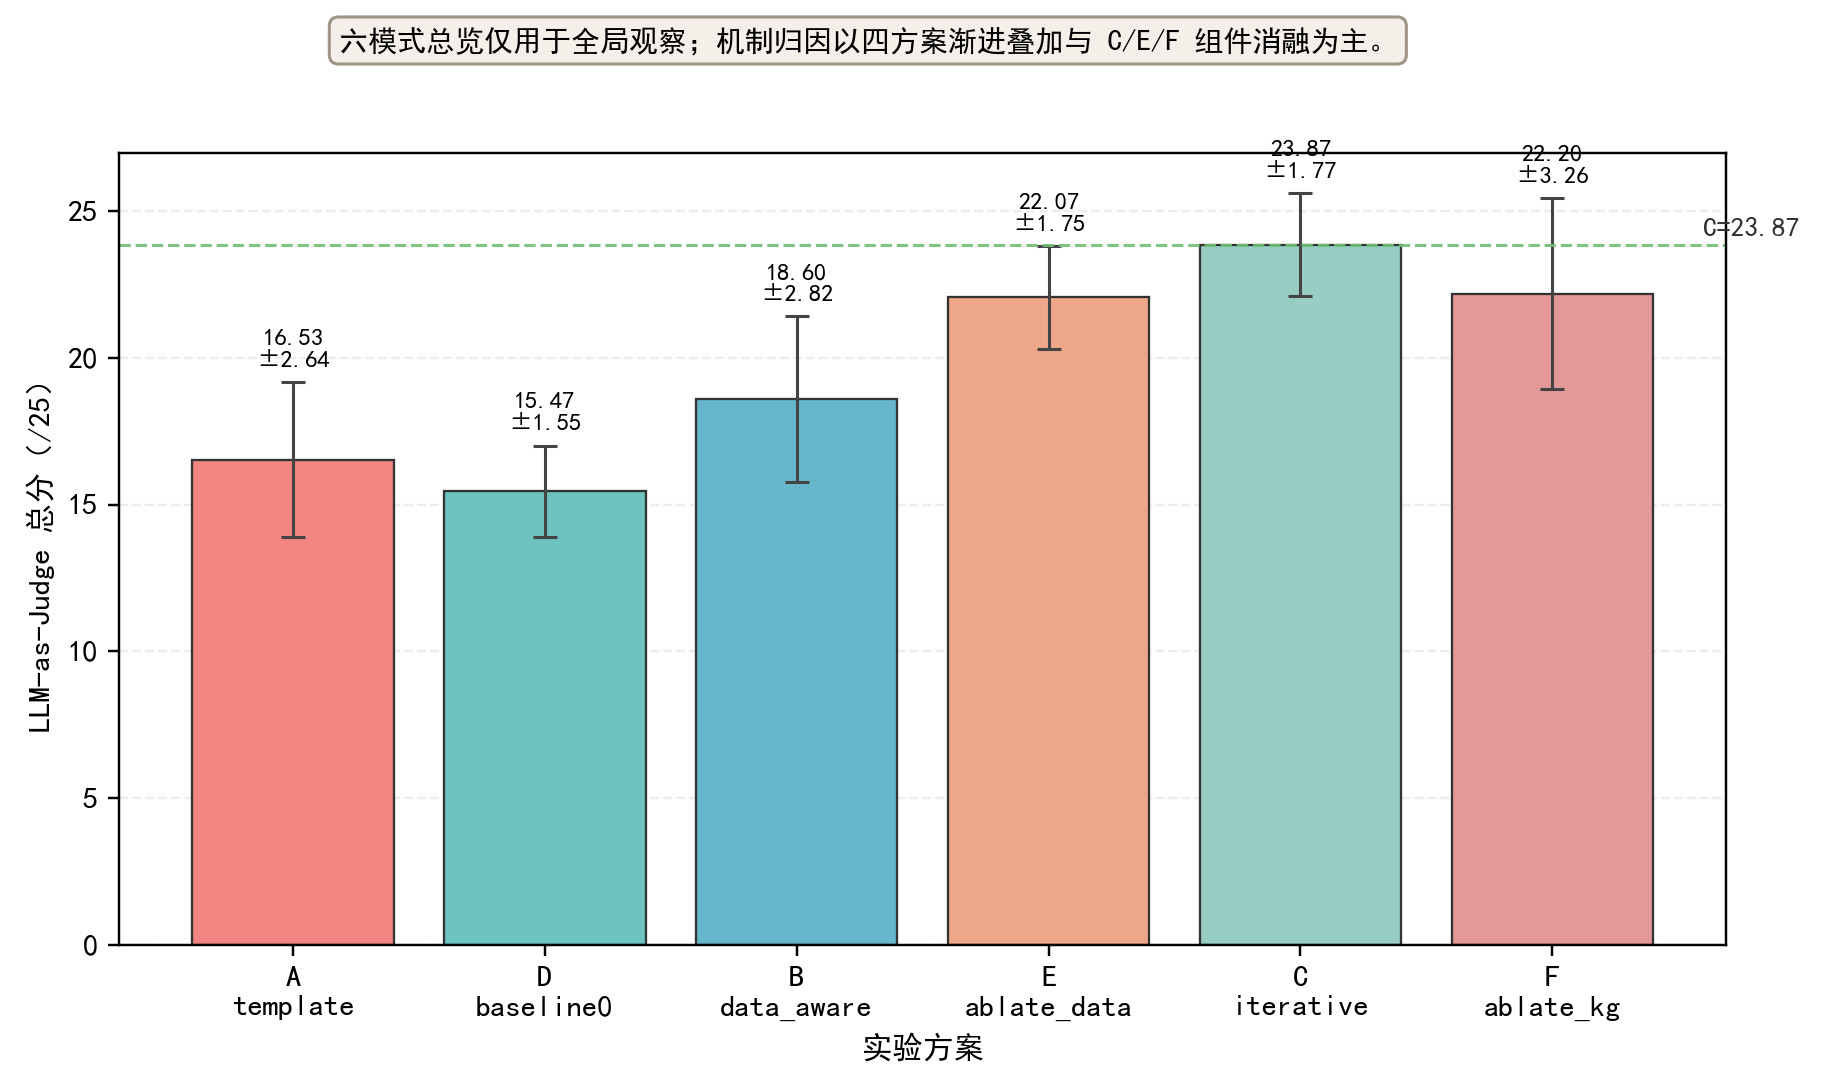
\includegraphics[width=0.78\textwidth]{figures/图5-2_六方案LLM总分柱状图.png}
\caption{六模式 LLM 总分总览（重复实验均值，误差线为标准差）}
\label{fig:ch5-overview}
\end{figure}

如图 \ref{fig:ch5-overview} 所示，六模式总览呈现出清晰分层：C\_iterative 的平均总分最高（23.87 $\pm$ 1.77），E\_ablate\_data 与 F\_ablate\_kg 处于第二梯队（分别为 22.07 $\pm$ 1.75 和 22.20 $\pm$ 3.26），B\_data\_aware 处于中间位置（18.60 $\pm$ 2.82），A\_template 与 D\_baseline0 则处于相对较低且彼此接近的区间（16.53 $\pm$ 2.64 和 15.47 $\pm$ 1.55）。这一总览说明完整系统在平均意义上最优，但六模式并列图本身只用于全局观察，不直接承担模块归因任务；系统为何变好以及各组件如何起作用，仍需回到渐进叠加和消融比较中分别解释。

\subsubsection{四方案渐进叠加主实验}

主实验关注 D\_baseline0、A\_template、B\_data\_aware 和 C\_iterative 四种模式。其核心目标不是给出单一排行榜，而是解释知识约束、数据感知与迭代优化如何逐步改变方案生成质量。

\begin{figure}[H]
\centering
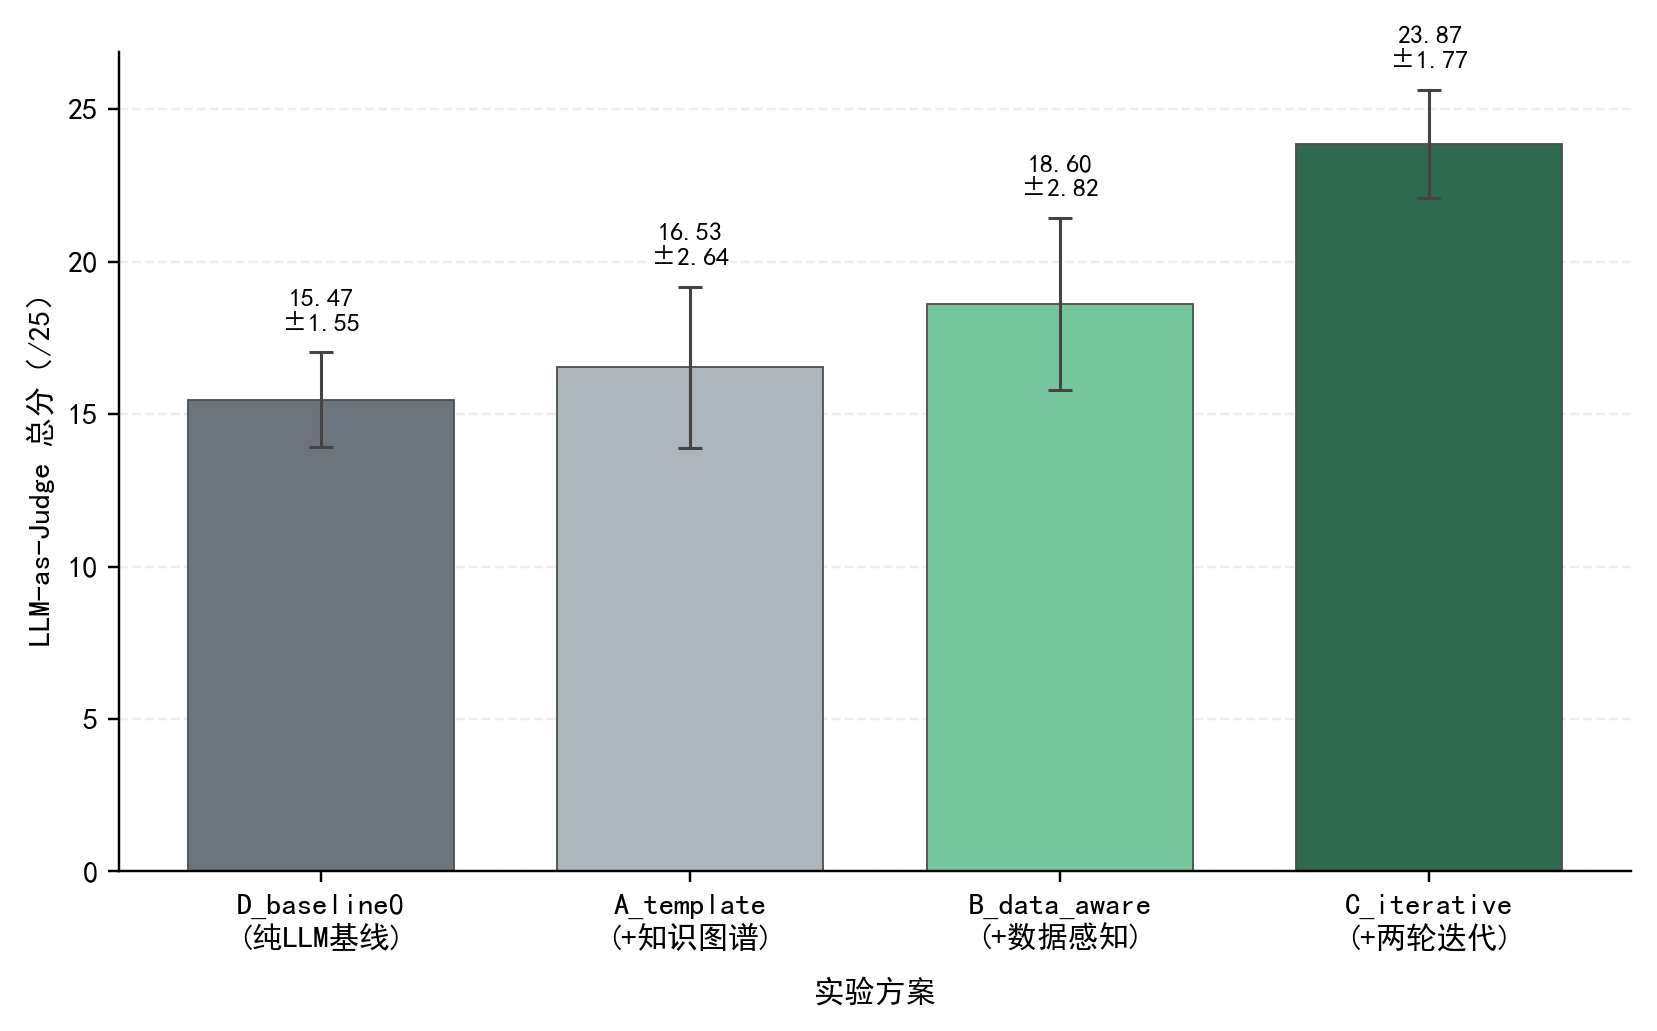
\includegraphics[width=0.72\textwidth]{figures/图5-1_四方案LLM总分柱状图.png}
\caption{四方案 LLM 总分对比（重复实验均值，误差线为标准差）}
\label{fig:ch5-main-total}
\end{figure}

\begin{table}[htbp]
\centering
\caption{四方案自动化指标对比（3 问题 $\times$ 5 次重复的均值 $\pm$ 标准差）}
\label{tab:main-auto}
\resizebox{\textwidth}{!}{
\begin{tabular}{lcccc}
\toprule
指标 & D\_baseline0 & A\_template & B\_data\_aware & C\_iterative \\
\midrule
数据列覆盖率 & 0.255 $\pm$ 0.051 & 0.276 $\pm$ 0.056 & 0.285 $\pm$ 0.053 & 0.358 $\pm$ 0.089 \\
方法多样性 & 2.667 $\pm$ 0.617 & 2.800 $\pm$ 0.561 & 2.667 $\pm$ 0.488 & 5.000 $\pm$ 0.655 \\
任务描述详细度 & 54.733 $\pm$ 20.518 & 55.627 $\pm$ 18.442 & 61.693 $\pm$ 18.554 & 85.167 $\pm$ 13.927 \\
针对性引用数 & 1.067 $\pm$ 1.100 & 1.200 $\pm$ 1.656 & 10.200 $\pm$ 4.161 & 14.200 $\pm$ 6.527 \\
控制变量数 & 1.733 $\pm$ 1.486 & 1.200 $\pm$ 1.207 & 0.400 $\pm$ 0.828 & 0.733 $\pm$ 0.961 \\
参数丰富度 & 6.333 $\pm$ 1.988 & 4.867 $\pm$ 1.552 & 5.133 $\pm$ 2.416 & 11.733 $\pm$ 3.240 \\
预期结论具体度 & 0.267 $\pm$ 0.320 & 0.300 $\pm$ 0.414 & 0.744 $\pm$ 0.288 & 0.427 $\pm$ 0.204 \\
数据洞察数量 & 0.000 $\pm$ 0.000 & 0.000 $\pm$ 0.000 & 2.800 $\pm$ 0.414 & 2.667 $\pm$ 0.816 \\
生成任务总数 & 2.800 $\pm$ 0.561 & 2.933 $\pm$ 0.458 & 2.800 $\pm$ 0.414 & 5.000 $\pm$ 0.655 \\
代码执行成功率 & 1.000 $\pm$ 0.000 & 1.000 $\pm$ 0.000 & 1.000 $\pm$ 0.000 & 1.000 $\pm$ 0.000 \\
\bottomrule
\end{tabular}
}
\vspace{0.3em}
\begin{minipage}{0.96\linewidth}
\footnotesize\raggedright
注：表中数值来自 3 个问题、每个问题 5 次重复实验的聚合结果；“控制变量数”受参数字段命名风格影响较大，仅作辅助观察。
\end{minipage}
\end{table}

\begin{table}[htbp]
\centering
\caption{四方案 LLM-as-Judge 评分对比（3 问题 $\times$ 5 次重复的均值 $\pm$ 标准差）}
\label{tab:main-llm}
\resizebox{\textwidth}{!}{
\begin{tabular}{lcccc}
\toprule
维度 & D\_baseline0 & A\_template & B\_data\_aware & C\_iterative \\
\midrule
相关性 & 3.73 $\pm$ 0.46 & 3.93 $\pm$ 0.46 & 4.07 $\pm$ 0.59 & 4.93 $\pm$ 0.26 \\
针对性 & 3.00 $\pm$ 0.00 & 3.40 $\pm$ 0.63 & 3.87 $\pm$ 0.83 & 4.73 $\pm$ 0.46 \\
方法合理性 & 3.27 $\pm$ 0.46 & 3.33 $\pm$ 0.62 & 3.40 $\pm$ 0.83 & 4.73 $\pm$ 0.46 \\
创新性 & 2.47 $\pm$ 0.52 & 3.20 $\pm$ 0.86 & 4.13 $\pm$ 0.52 & 4.73 $\pm$ 0.46 \\
深度 & 3.00 $\pm$ 0.54 & 2.67 $\pm$ 0.62 & 3.13 $\pm$ 0.74 & 4.73 $\pm$ 0.46 \\
总分(/25) & 15.47 $\pm$ 1.55 & 16.53 $\pm$ 2.64 & 18.60 $\pm$ 2.82 & 23.87 $\pm$ 1.77 \\
\bottomrule
\end{tabular}
}
\end{table}

\begin{figure}[H]
\centering
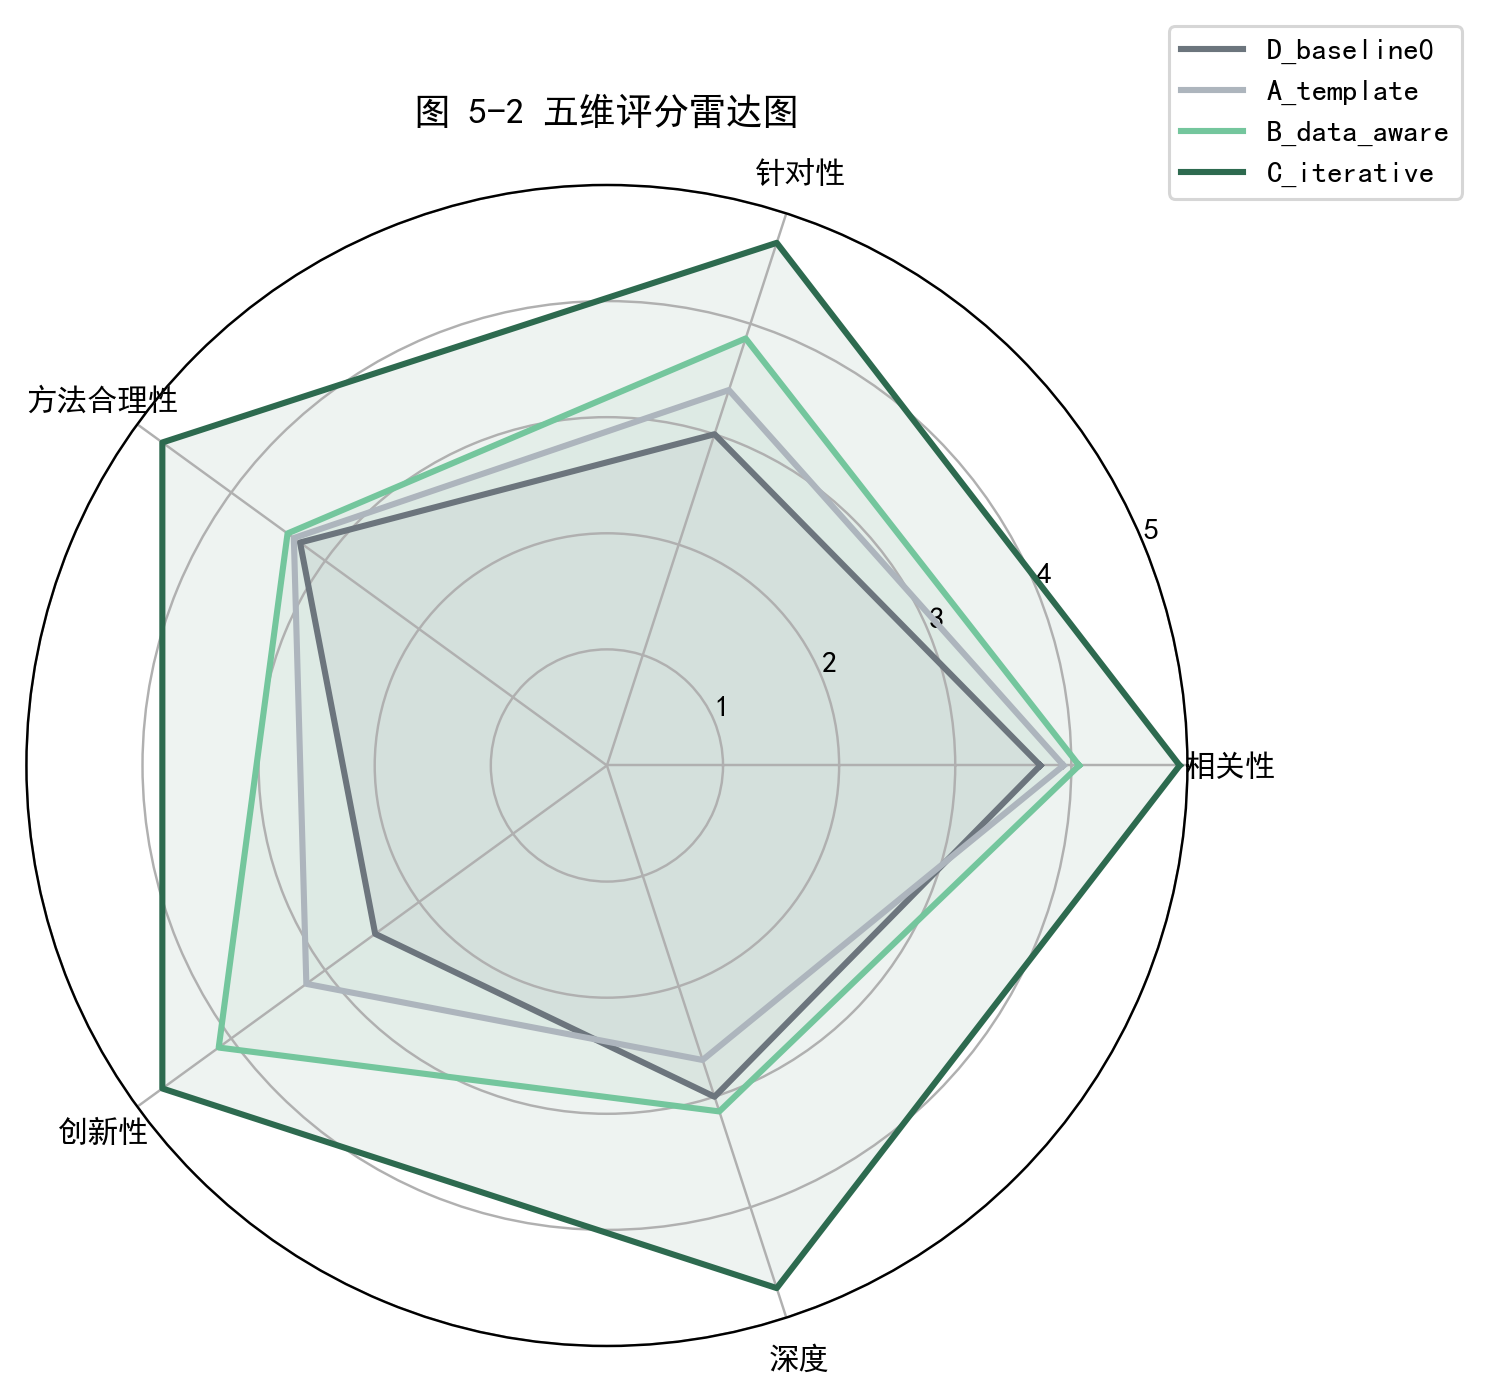
\includegraphics[width=0.68\textwidth]{figures/图5-2_五维评分雷达图.png}
\caption{四方案五维语义评分雷达图（重复实验均值）}
\label{fig:ch5-main-radar}
\end{figure}

\begin{figure}[H]
\centering
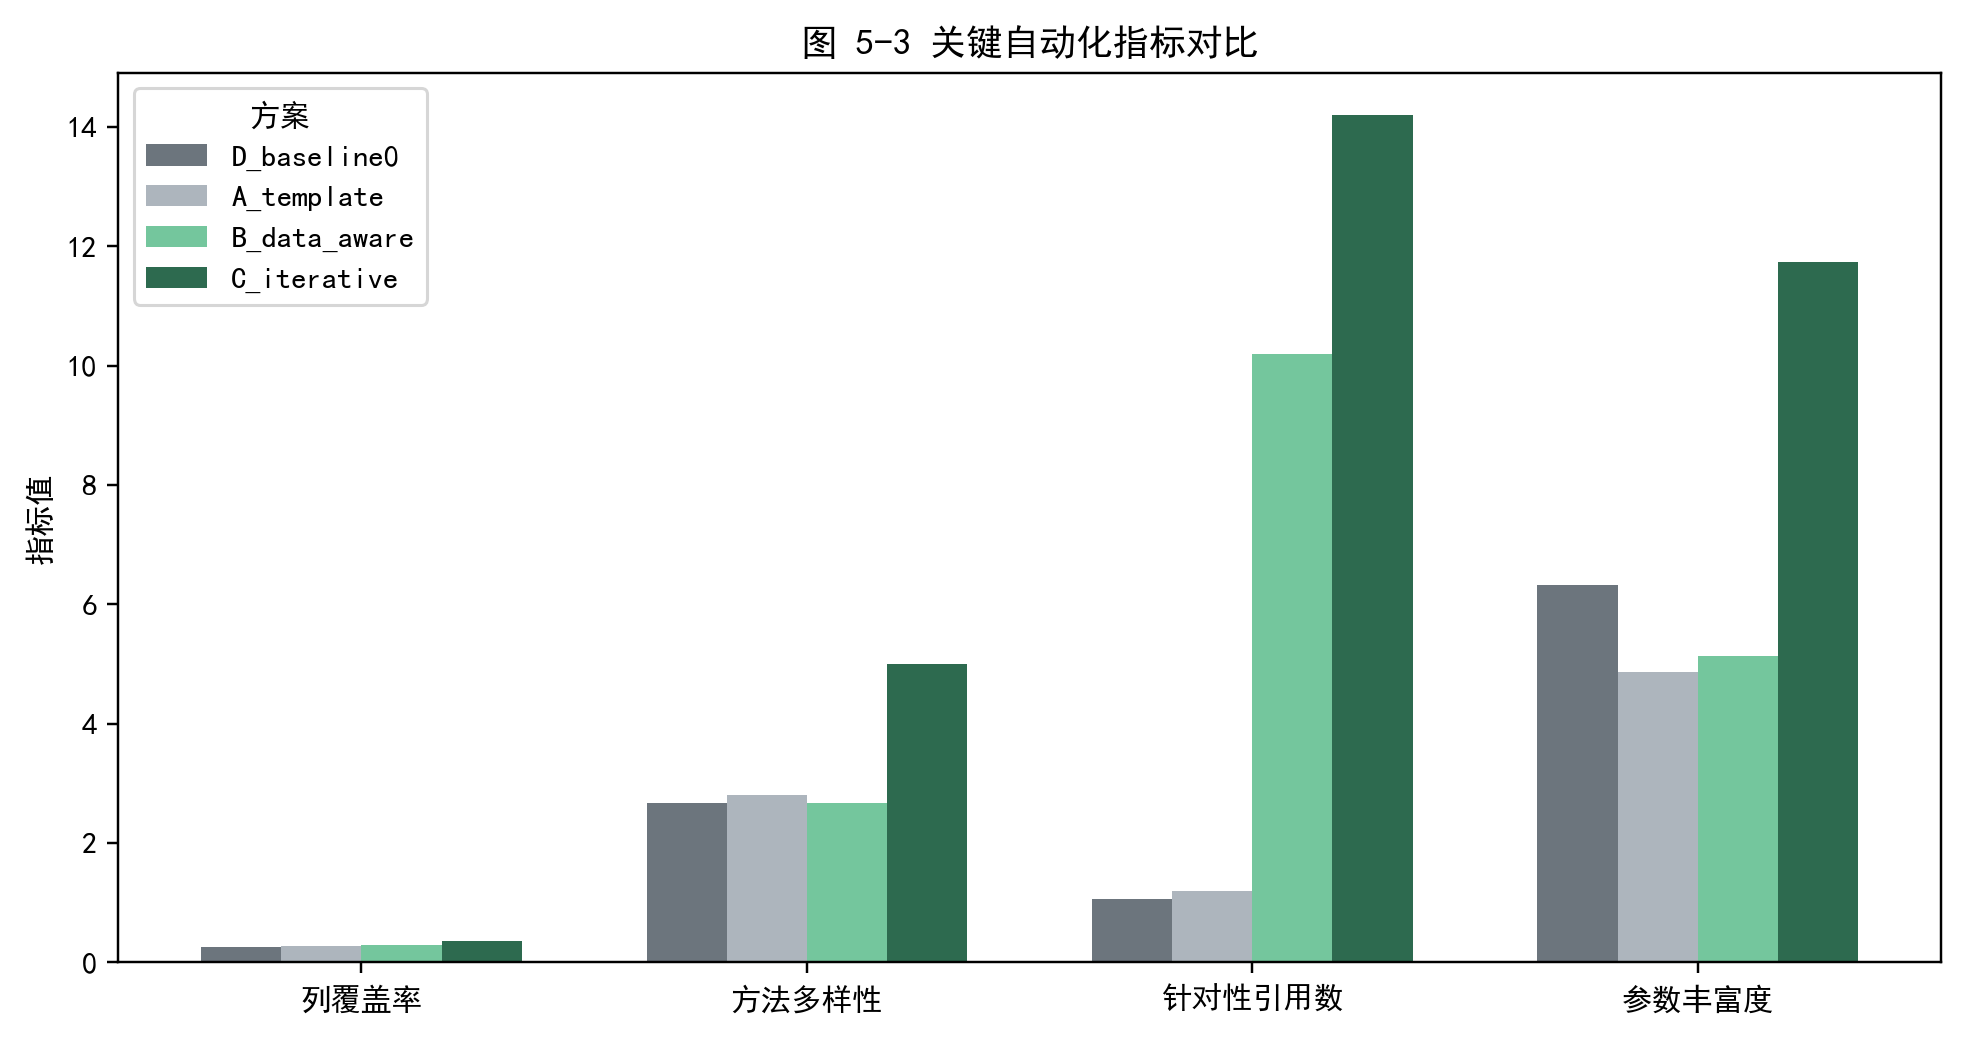
\includegraphics[width=0.84\textwidth]{figures/图5-3_自动化指标对比图.png}
\caption{四方案关键自动化指标对比（重复实验均值）}
\label{fig:ch5-main-auto}
\end{figure}

\begin{table}[htbp]
\centering
\caption{四方案问题级 LLM 总分明细（均值 $\pm$ 标准差）}
\label{tab:main-question}
\resizebox{\textwidth}{!}{
\begin{tabular}{lcccc}
\toprule
研究问题 & D\_baseline0 & A\_template & B\_data\_aware & C\_iterative \\
\midrule
Q1 技术影响力驱动因素 & 16.20 $\pm$ 2.05 & 17.00 $\pm$ 1.87 & 19.60 $\pm$ 1.95 & 22.20 $\pm$ 2.17 \\
Q2 技术融合趋势识别 & 15.20 $\pm$ 0.84 & 16.80 $\pm$ 4.03 & 17.40 $\pm$ 2.51 & 24.60 $\pm$ 0.89 \\
Q3 国家竞争态势评估 & 15.00 $\pm$ 1.58 & 15.80 $\pm$ 1.92 & 18.80 $\pm$ 3.83 & 24.80 $\pm$ 0.45 \\
\bottomrule
\end{tabular}
}
\end{table}

图 \ref{fig:ch5-main-total} 和表 \ref{tab:main-llm} 给出了主实验的核心结论。首先，C\_iterative 在四方案中显著领先，总分达到 23.87 $\pm$ 1.77，明显高于 B\_data\_aware 的 18.60 $\pm$ 2.82，也远高于 A\_template 与 D\_baseline0。其次，B\_data\_aware 稳定高于 A\_template 与 D\_baseline0，尤其在针对性、创新性和总分维度上体现出较清晰的领先。再次，A\_template 与 D\_baseline0 的均值差距相对有限：A 在相关性、针对性、方法合理性和创新性上略高于 D，但在深度维度仍低于 D，说明仅凭知识模板约束并不足以稳定拉开性能差距，其主要作用更接近“提供结构先验”而非“直接带来全面提升”。

自动化结构指标进一步解释了上述语义差异。表 \ref{tab:main-auto} 和图 \ref{fig:ch5-main-auto} 表明，完整模式 C 在列覆盖率、方法多样性、参数丰富度、任务总数和针对性引用数等关键指标上均处于显著领先位置，说明两轮迭代不仅增加了任务数量，更实质性地扩展了方法空间与证据引用密度。与单次实验版本不同，重复实验中的 B\_data\_aware 并未表现出“列覆盖率下降”的稳定特征，其列覆盖率均值（0.285）略高于 D\_baseline0（0.255），任务总数也基本相近（2.800 vs 2.800），但针对性引用数由 1.067 提升到 10.200。这说明数据感知在重复实验中表现出的主要效果不是“以广度换深度”，而是让系统在保持基础覆盖的同时更频繁地围绕真实数据证据组织任务。

从问题级结果看，三类研究问题对各增强模块的敏感性存在明显差异。Q2 中，C\_iterative 以 24.60 $\pm$ 0.89 显著领先其余三种模式，说明在同时需要整合图结构信号、文本语义与多步任务编排的结构—趋势类问题上，数据感知与迭代机制几乎是决定上限的必要条件。Q1 和 Q3 中，A 与 D 的差距均相对有限，而 B 和 C 的优势更加清晰，说明数据证据注入对开放问题的帮助更直接。总体上，主实验支持两个稳健判断：第一，数据感知是把系统从“纯语义规划”推进到“证据驱动规划”的关键机制；第二，两轮迭代是进一步把中等质量方案提升为高质量方案的核心环节。

\subsubsection{组件消融实验}

前述 D$\rightarrow$A$\rightarrow$B$\rightarrow$C 主实验解释了系统为何随着模块叠加而变好，但无法直接回答“在完整系统中，若单独移除某个组件，会造成多大影响”这一问题。为此，本文在 C\_iterative 的基础上设计了 E\_ablate\_data 和 F\_ablate\_kg 两组消融，用于分别考察数据感知和知识图谱的独立贡献。

\begin{table}[htbp]
\centering
\caption{组件消融自动化指标对比（3 问题 $\times$ 5 次重复的均值 $\pm$ 标准差）}
\label{tab:ablation-auto}
\resizebox{\textwidth}{!}{
\begin{tabular}{lccc}
\toprule
指标 & C\_iterative & E\_ablate\_data & F\_ablate\_kg \\
\midrule
数据列覆盖率 & 0.358 $\pm$ 0.089 & 0.349 $\pm$ 0.082 & 0.345 $\pm$ 0.062 \\
方法多样性 & 5.000 $\pm$ 0.655 & 4.533 $\pm$ 0.640 & 4.933 $\pm$ 0.961 \\
任务描述详细度 & 85.167 $\pm$ 13.927 & 83.853 $\pm$ 17.473 & 89.313 $\pm$ 28.003 \\
针对性引用数 & 14.200 $\pm$ 6.527 & 3.000 $\pm$ 2.752 & 14.533 $\pm$ 6.917 \\
参数丰富度 & 11.733 $\pm$ 3.240 & 11.467 $\pm$ 1.959 & 11.533 $\pm$ 2.642 \\
数据洞察数量 & 2.667 $\pm$ 0.816 & 0.000 $\pm$ 0.000 & 2.600 $\pm$ 1.056 \\
生成任务总数 & 5.000 $\pm$ 0.655 & 4.867 $\pm$ 0.516 & 4.867 $\pm$ 0.640 \\
代码执行成功率 & 1.000 $\pm$ 0.000 & 1.000 $\pm$ 0.000 & 1.000 $\pm$ 0.000 \\
\bottomrule
\end{tabular}
}
\end{table}

\begin{table}[htbp]
\centering
\caption{组件消融 LLM-as-Judge 评分对比（3 问题 $\times$ 5 次重复的均值 $\pm$ 标准差）}
\label{tab:ablation-llm}
\resizebox{\textwidth}{!}{
\begin{tabular}{lccc}
\toprule
维度 & C\_iterative & E\_ablate\_data & F\_ablate\_kg \\
\midrule
相关性 & 4.93 $\pm$ 0.26 & 4.73 $\pm$ 0.46 & 4.67 $\pm$ 0.62 \\
针对性 & 4.73 $\pm$ 0.46 & 4.33 $\pm$ 0.49 & 4.73 $\pm$ 0.59 \\
方法合理性 & 4.73 $\pm$ 0.46 & 4.53 $\pm$ 0.52 & 4.20 $\pm$ 0.68 \\
创新性 & 4.73 $\pm$ 0.46 & 3.87 $\pm$ 0.35 & 4.40 $\pm$ 0.91 \\
深度 & 4.73 $\pm$ 0.46 & 4.60 $\pm$ 0.51 & 4.20 $\pm$ 0.78 \\
总分(/25) & 23.87 $\pm$ 1.77 & 22.07 $\pm$ 1.75 & 22.20 $\pm$ 3.26 \\
\bottomrule
\end{tabular}
}
\end{table}

\begin{table}[htbp]
\centering
\caption{组件消融问题级 LLM 总分明细（均值 $\pm$ 标准差）}
\label{tab:ablation-question}
\resizebox{\textwidth}{!}{
\begin{tabular}{lccc}
\toprule
研究问题 & C\_iterative & E\_ablate\_data & F\_ablate\_kg \\
\midrule
Q1 技术影响力驱动因素 & 22.20 $\pm$ 2.17 & 21.20 $\pm$ 1.64 & 24.60 $\pm$ 0.89 \\
Q2 技术融合趋势识别 & 24.60 $\pm$ 0.89 & 22.40 $\pm$ 1.95 & 21.40 $\pm$ 1.52 \\
Q3 国家竞争态势评估 & 24.80 $\pm$ 0.45 & 22.60 $\pm$ 1.67 & 20.60 $\pm$ 4.78 \\
\bottomrule
\end{tabular}
}
\end{table}

从平均结果看，C\_iterative 在消融比较中仍保持最高总分（23.87 $\pm$ 1.77），高于 E\_ablate\_data 的 22.07 $\pm$ 1.75 和 F\_ablate\_kg 的 22.20 $\pm$ 3.26。这一结果与单次实验版本中“移除知识图谱后总体更好”的观察不同，表明在重复实验口径下，完整系统的平均优势是可以复现的。

对比 C 与 E，可以较清晰地观察到数据感知模块的直接贡献。表 \ref{tab:ablation-auto} 显示，移除数据感知后，针对性引用数由 14.200 大幅降至 3.000，数据洞察数量由 2.667 变为 0，方法多样性和任务总数也同步下降；表 \ref{tab:ablation-llm} 则显示，E 在针对性、创新性和总分上均低于 C。说明 DataPreview 和 GraphPreview 并非仅增加上下文长度，而是实质改变了任务设计的出发点，使系统能够围绕当前数据中已经显露的模式组织分析路径。

对比 C 与 F，可以更细致地理解知识图谱的任务依赖性。平均结果上，F 的总分低于 C，说明知识图谱在整体上仍提供了正向作用；但表 \ref{tab:ablation-question} 同时表明，这一收益并不均匀。Q1 中，F 以 24.60 $\pm$ 0.89 高于 C 的 22.20 $\pm$ 2.17，说明在开放度更高、可由数据直接驱动多种解释路径的问题上，移除静态图谱约束可能释放更多探索空间。相反，Q2 和 Q3 中，C 分别以 24.60 $\pm$ 0.89 和 24.80 $\pm$ 0.45 明显高于 F 的 21.40 $\pm$ 1.52 和 20.60 $\pm$ 4.78，说明当问题具有较清晰的结构锚点、需要多步链式分析时，知识图谱能够更稳定地约束变量选择与方法路径，从而提升方案质量。

综合主实验与消融实验可以得到如下机制解释：数据感知回答“当前数据最值得看什么”，知识图谱回答“面对这类证据通常该怎么分析”，两轮迭代则负责“发现第一轮不足后如何继续深化”。三者共同组成了完整系统的性能来源。若只保留其中任意两个组件，系统仍可得到较高分数；但若要在多种问题上同时保持高针对性、高方法合理性和高深度，完整配置仍然最稳。

\subsubsection{有效性威胁与缓解}

第一，\textbf{统计显著性仍待补充}。本文已经对 6 种模式、3 个问题各独立重复运行 5 次，显著降低了单次观察带来的偶然性风险，但尚未进一步对关键差异进行正式显著性检验。因此，当前结论可被视为“具有重复证据支持的稳健趋势”，后续仍需通过 bootstrap 置信区间、Friedman 检验或 Wilcoxon 符号秩检验补充统计推断。

第二，\textbf{评估主体单一}。LLM-as-Judge 虽采用匿名并列评分和低温度参数缓解偏差，但仍可能偏好某些表述风格、方法路径或文本长度。本文通过在同一“问题 × 重复轮次”内混排六种方案降低标签干扰，但从方法论上看，后续仍应加入人工专家盲审或多模型集成评分作为交叉校验。

第三，\textbf{问题集规模有限}。当前仅覆盖三个研究问题，虽分别代表解释型、结构—趋势型和比较评估型任务，但在统计外推和任务多样性方面仍然有限。后续需扩展问题库并在更多数据集上复验关键结论，以提高外部有效性。

第四，\textbf{实现配置依赖}。本文控制了统一模型版本、提示模板和执行环境，使相对比较更具可比性，但不同模型、不同提示配置和不同计算环境下是否仍保持类似排序，仍需后续补充验证。

\subsection{本章小结}

本章采用“六模式总览 + 四方案渐进叠加主实验 + 组件消融”的组织方式，对 90 组重复实验结果进行了系统分析。总体来看，C\_iterative 是当前最优且最稳定的配置；B\_data\_aware 稳定优于 A\_template 与 D\_baseline0，说明数据感知是推动方案从语义驱动走向证据驱动的关键机制；知识图谱在平均意义上提供正向贡献，但收益强度具有明显任务依赖性。与单次实验相比，重复实验使本文的结论从“初始观察”转化为“具有重复支持的机制判断”，为后续应用示例与总结章节提供了更稳健的实证基础。
